\documentclass{beamer}

%
% Tria l'aspecte de la teva presentació.
%
% Per més temes, temes de color i de fonts, consulta:
% http://deic.uab.es/~iblanes/beamer_gallery/index_by_theme.html
%
\mode<presentation>
{
  \usetheme{Warsaw}       % o prova Darmstadt, Madrid, Dresden, ...
  \usecolortheme{default} % o prova albatross, beaver, crane, ...
  \usefonttheme{default}  % o prova serif, structurebold, ...
  \setbeamertemplate{navigation symbols}{}
  \setbeamertemplate{caption}[numbered]
} 

\usepackage[english]{babel}
\usepackage[utf8]{inputenc}

\title{Ars Magna: El projecte}
\author{Ramon Llull}
\institute{Cort del Rei en Jaume II}
\date{19 novembre 1283}

\begin{document}

\begin{frame}
  \titlepage
\end{frame}

\begin{frame}{Guió}
  \tableofcontents
\end{frame}

\section{Ordre del dia}

\begin{frame}{Ordre del dia}

\begin{itemize}
  \item Missió 
  \item Visió
  \item Full de ruta
  \item Conclusions
\end{itemize}

\end{frame}



\section{Missió}

\begin{frame}{Missió}

\begin{block}{Missió}
\begin{itemize}
\item Convertir el infidels
  \begin{itemize}
    \item Jueus
    \item Gentils
  \end{itemize}
\item La força de la raó
\end{itemize}
\end{block}

\end{frame}

\begin{frame}{Visió}

\section{Visió}
\begin{block}{Visió}
\begin{itemize}
\item Escriure el millor llibre del món
\item Fer monestirs per aprendre llengües 
\item Reprendre les creuades
\end{itemize}
\end{block}

\end{frame}

\section{Full de ruta}

\begin{frame}{Full de ruta}

\begin{figure}
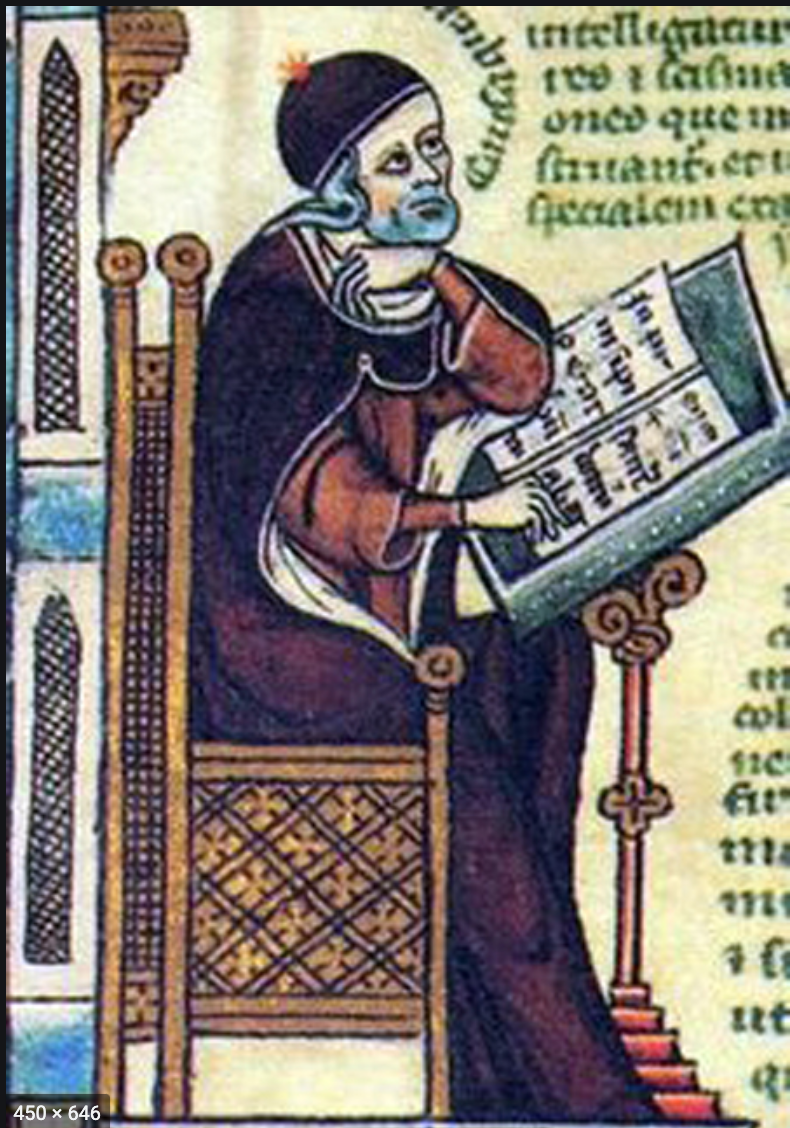
\includegraphics[width=0.2\textwidth]{llull}
\end{figure}

\begin{block}{Il·luminació}
D'acord amb una comunicació personal de Déu:
\begin{itemize}
\item La lògica ha de ser la base del llibre.
\item Nocions comuns a totes les religions.
\item Superar el mètode escolàstic.
\end{itemize}
\end{block}

\end{frame}

\begin{frame}{Taxa de conversions esperada}

\begin{center}
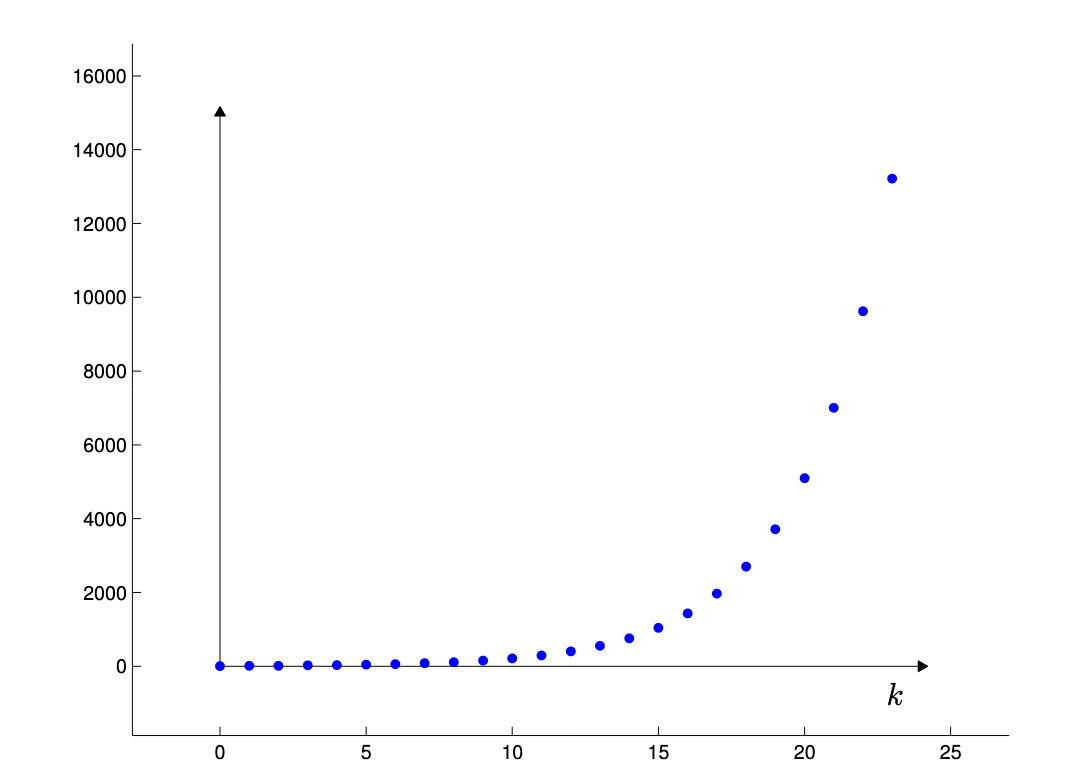
\includegraphics[scale=.25]{malthus}
\end{center}

\begin{equation}
\begin{pmatrix}x_{n+1} \\ x_n \end{pmatrix} = \begin{pmatrix}
3.5 &2 \\
1 & 0
\end{pmatrix}
\begin{pmatrix}
x_n \\
x_{n-1}
\end{pmatrix}
\end{equation}

\end{frame}

\begin{frame}{Fora de l'ordre del dia}

\begin{itemize}[<+->]
  \item Bondat
  \item Grandesa 
  \item Eternitat
  \item Poder
  \item Raó
  \item Voluntat
  \item Virtut
  \item Veritat
  \item Gloria
\end{itemize}

\end{frame}

\section{Conclusions}
\begin{frame}{Conclusions}

\begin{columns}
\begin{column}{0.4\textwidth}
\begin{itemize}
\item La raó
\item Més enllà de la fe
\item S'ha de predicar en la llengua dels infidels
\end{itemize}
\end{column}
\begin{column}{0.6\textwidth}
\begin{itemize}
\item Superar el mètode escolàstic
\item La lògica com a base
\item Les creuades per donar suport a tot plegat
\end{itemize}
\end{column}
\end{columns}

\end{frame}

\end{document}

